%!TeX root=./maximo.tex


\section{Heap cinético}\label{sec:heap-cinetico}
Um bom jeito de resolver o problema do máximo cinético é manter uma fila de
prioridades com os elementos da coleção tendo como prioridade o valor corrente
do elemento.
Dessa maneira, o elemento que se encontra na raiz da fila será o que possui o maior valor da
coleção.
Para implementar a fila utilizaremos um vetor organizado como um heap.

Inicialmente o vetor começa com os índices dos elementos e o reorganizamos como um
heap usando como chave o valor de cada elemento no instante $t = 0$, ou seja, o
valor $x_0$ de cada elemento.

Uma vez montado o heap, construímos um certificado para cada par $($filho,
pai$)$ no heap.
O $i$-ésimo certificado se refere ao par das posições $i$ e $\floor{\frac{i}{2}}$ e consiste no
instante de tempo em que o $i$-ésimo elemento passará a ter um valor maior que o valor do
$\floor{\frac{i}{2}}$-ésimo elemento do vetor, se esse instante for maior que o instante atual.
Do contrário, o certificado consiste em $+\infty$.

Esses $n - 1$ certificados são colocados em uma fila com prioridades $Q$, com o
prazo de validade como chave.
Estamos interessados nos certificados com menor prazo de validade.

Para descrever a implementação das três operações, precisamos estabelecer o nome
das novas variáveis usadas.
São elas:
\begin{enumerate}
    \item \textit{heap}: vetor com os índices dos $n$ elementos
    formando um heap de acordo com o seu valor no instante
    \textit{now};
    \item \textit{cert}: vetor com os certificados, onde
    \textit{cert}$[i]$ guarda o certificado entre $i$ e
    $\floor{\frac{i}{2}}$, para $1 < i \leq n$.
\end{enumerate}

A interface da fila com prioridades que utilizaremos não se altera.

Um evento está associado a um certificado $(i, t)$ que expira no instante $t$,
como pode ser visto na Figura~\ref{fig:maxdevent}.
O tratamento do evento correspondente ao certificado $(i, t)$ consiste em trocar de lugar os
índices armazenados nas posições $i$ e $\floor{\frac{i}{2}}$ do vetor \heap, e recalcular o prazo
de validade de até cinco certificados, ilustrados na Figura~\ref{fig:max:update}:
\begin{itemize}
    \item do $\floor{\frac{i}{2}}$-ésimo certificado, se $i > 1$;
    \item do $j$-ésimo certificado, se $i > 1$ e $j \leq n$,
    onde $j = 2\cdot \floor{\frac{i}{2}} + ((i + 1)\mod2)$
    é o irmão de $i$;
    \item do $(2i)$-ésimo certificado, se $2i \leq n$;
    \item do $(2i + 1)$-ésimo certificado, se $2i + 1 \leq n$.
\end{itemize}

\begin{table}[htb]
    \begin{tabular}{|c|c|c|c|c|}
        \hline
        &       &       & $\now = 0$ & $\now = 1$ \\
        $i$   & $x_0$ & $v$   & $\cert[i]$ & $\cert[i]$ \\
        \hline
        $1$   & $2$   & $2$   & $?$        & $?$        \\

        $2$   & $6$   & $1$   & $?$        & $?$        \\

        $3$   & $-6$  & $3$   & $?$        & $?$        \\

        $4$   & $-16$ & $4$   & $?$        & $?$        \\

        $5$   & $-1$  & $5$   & $?$        & $?$        \\

        $6$   & $1$   & $2.5$ & $?$        & $?$        \\

        $7$   & $-18$ & $6$   & $?$        & $?$        \\

        $8$   & $5$   & $1$   & $?$        & $?$        \\

        % $9$ & $-12$ & $3$ & $?$ & $?$ \\
        \hline
    \end{tabular}
    \caption{Tabela para as Figuras~\ref{fig:maxdevent}
    e~\ref{fig:max:update}. (incompleta)}\label{tab:table}
\end{table}

O $i$-ésimo certificado também deve ser ajustado para $+\infty$.
Finalmente, é necessário fazer ajustes em $Q$, alterando a chave dos certificados que sofreram
alteração.

\begin{table}[htb]
    \begin{tabular}{|c|c|c|c|c|}
        \hline
        &       &       & $\now = 0$ & $\now = 1$ \\
        $i$   & $x_0$ & $v$   & $\cert[i]$ & $\cert[i]$ \\
        \hline
        $1$   & $2$   & $2$   & $?$        & $?$        \\

        $2$   & $6$   & $1$   & $?$        & $?$        \\

        $3$   & $-6$  & $3$   & $?$        & $?$        \\

        $4$   & $-16$ & $4$   & $?$        & $?$        \\

        $5$   & $-1$  & $5$   & $?$        & $?$        \\

        $6$   & $1$   & $2.5$ & $?$        & $?$        \\

        $7$   & $-18$ & $6$   & $?$        & $?$        \\

        $8$   & $5$   & $1$   & $?$        & $?$        \\

        % $9$ & $-12$ & $3$ & $?$ & $?$ \\
        \hline
    \end{tabular}
    \caption{Tabela para as Figuras~\ref{fig:maxdevent}
    e~\ref{fig:max:update}. (incompleta)}\label{tab:table}
\end{table}

Novamente, na implementação da operação \textsc{event}, no Algoritmo~\ref{max:evento},
utilizaremos a rotina \textsc{update}$(i)$, do Algoritmo~\ref{max:update}, que calcula a nova
validade $t$ do $i$-ésimo certificado, se $1 < i \leq n$, e chama a rotina \textsc{updatePQ}$(Q, i,
t)$.

\begin{algorithm}
    \caption{Função \textsc{update}.} \label{lista:update}
\begin{algorithmic}[1]
    \Function{update}{$i$}
        \If{$1 \leq i < n$}
            \State $t \leftarrow $ \Call{expire}{$i,i+1$}
            \State \Call{updatePQ}{$Q,i,t$}
        \EndIf
    \EndFunction
\end{algorithmic}
\end{algorithm}

\begin{algorithm}
    \caption{Função \textsc{event}.} \label{torneioi:evento}
    \begin{algorithmic}[1]
        \Function{event}{\nnull}
            \State $e \leftarrow  $ \Call{minPQ}{$Q$}
            \While{$e.\cert$ = \now}
                \State $j \leftarrow e.\lastmatch$
                \State $k \leftarrow 2\cdot \floor{\frac{j}{2}}
                + ((j + 1)\mod2)$ \Comment{adversário}
                \While{$j > 1$ \AND \Call{compare}{$j, k$}}
                    \State \torneio[$\floor{\frac{j}{2}}$]
                    $\leftarrow~$\torneio[$j$]
                    \State $\torneio[k].\lastmatch$ $\leftarrow k$
                    \State \Call{update}{$\torneio[k]$}
                    \State $j \leftarrow \floor{\frac{j}{2}}$
                    \State $k \leftarrow 2\cdot \floor{\frac{j}{2}}
                    + ((j + 1)\mod2)$ \Comment{adversário}
                \EndWhile
                \State $\torneio[j].\lastmatch \leftarrow j$
                \State \Call{update}{$\torneio[j]$}
                \State $e \leftarrow  $ \Call{minPQ}{$Q$}
            \EndWhile
        % \LineComment{swapHeap$(i, \floor{\frac{i}{2}})$ troca \heap[$i$] por \heap$\left[\floor{\frac{i}{2}}\right]$}
        \EndFunction
        \LineComment{\Call{compare}{$i, j$} retorna se o valor
        de $i$ é maior que o valor de $j$.}
    \end{algorithmic}
\end{algorithm}

A operação \textsc{query\_max}$()$, no Algoritmo~\ref{max:heap:querymax},
consiste em devolver \textit{heap}$[1]$, enquanto que a operação
\textsc{change}$(j, v)$, no Algoritmo~\ref{alg:heap:change}, consiste em alterar
a posição $x_0[j]$ para ${x_0[j] + (\mathit{speed}[j] - v)\cdot now}$, a posição
\textit{speed}[j] para \textit{v} e recalcular os eventuais certificados de que
$j$ participa.
Para tanto, a partir da posição $i$ em que $j$ se encontra no vetor \textit{heap}, podemos
recalcular \textit{cert}$[i]$ se $i > 1$, \textit{cert}$[2i]$ se $2i \leq n$ e \textit{cert}$[2i +
1]$ se $2i + 1 \leq n$, acionando a rotina \textsc{update} para fazer os devidos acertos em $Q$
correspondentes a estas modificações.
Veja a Figura~\ref{fig:predeventheap}.

\begin{figure}[H]
    \centering
    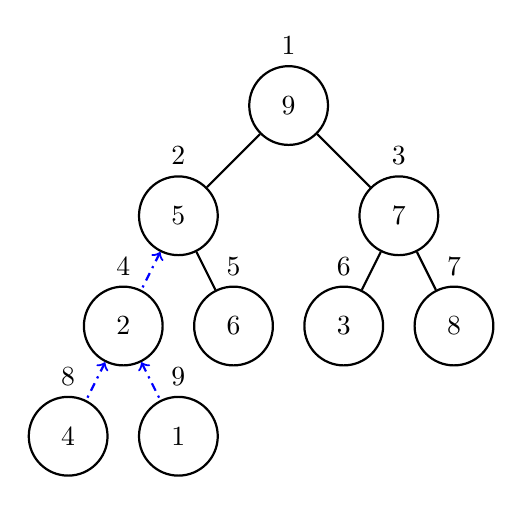
\begin{tikzpicture}[thick, scale=0.7]
        \node[label={1},circle,draw,minimum size=1cm]
        (1) at (0,0) {$9$};
        \node[label={2},circle,draw,minimum size=1cm]
        (2) at (-2,-2) {$5$};
        \node[label={3},circle,draw,minimum size=1cm]
        (3) at (2,-2) {$7$};
        \node[label={4},circle,draw,minimum size=1cm]
        (4) at (-3,-4) {$2$};
        \node[label={5},circle,draw,minimum size=1cm]
        (5) at (-1,-4) {$6$};
        \node[label={6},circle,draw,minimum size=1cm]
        (6) at (1,-4) {$3$};
        \node[label={7},circle,draw,minimum size=1cm]
        (7) at (3,-4) {$8$};
        \node[label={8},circle,draw,minimum size=1cm]
        (8) at (-4,-6) {$4$};
        \node[label={9},circle,draw,minimum size=1cm]
        (9) at (-2,-6) {$1$};

        \tikzstyle{cert}=[<-, dashdotted, blue, thick]
        \draw[thick] (1) -- (2);
        \draw[thick] (1) -- (3);
        \draw[cert] (2) -- (4);
        \draw[thick] (2) -- (5);
        \draw[thick] (3) -- (6);
        \draw[thick] (3) -- (7);
        \draw[cert] (4) -- (8);
        \draw[cert] (4) -- (9);
    \end{tikzpicture}
    \caption[Exemplo certificados do heap cinético após operação \textsc{change}]{Após a mudança de
    velocidade do elemento 2, que se encontra em \heap[$4$], os certificados
    \cert[$4$], \cert[$8$] e \cert[$9$] foram atualizados.}
    \label{fig:predeventheap}
\end{figure}

\begin{algorithm}
    \caption{Função \textsc{query\_max}.} \label{torn:querymax}
    \begin{algorithmic}[1]
        \Function{query\_max}{\null}
            \State \Return \torneio$[1]$
        \EndFunction
    \end{algorithmic}
\end{algorithm}

\begin{algorithm}
    \caption{Função \textsc{change}.} \label{torneioi:change}
    \begin{algorithmic}[1]
        \Function{change}{$j, v$}
            \State $e \leftarrow$ \Call{getObject}{$j$}
            \State $e.x_0 \leftarrow e.x_0+~(e.\speed -~v)~\cdot~\now$;
            \State $e.\speed \leftarrow v$
            \State $i \leftarrow e.\lastmatch$
            \State \Call{update}{$e$}
            \While{$i < n$}
                \If{$\torneio[i] = \torneio[2i]$}
                    \State $i \leftarrow 2i$
                \Else
                    \State $i \leftarrow 2i + 1$
                \EndIf
                \State $k \leftarrow 2\cdot \floor{\frac{i}{2}}
                + ((i + 1)\mod2)$ \Comment{adversário}
                \State \Call{update}{$\torneio[k]$}
            \EndWhile
        \EndFunction
    \end{algorithmic}
\end{algorithm}

\FloatBarrier

\subsection{Análise de desempenho}\label{subsec:heap:analise-de-desempenho}

O heap cinético é uma estrutura \textit{responsiva}, pois o custo de processar
um certificado é $O(\lg{n})$, onde $n$ é a quantidade de pontos.
O custo de processar um certificado corresponde a uma iteração da linha $3$ da operação
\textsc{event}, que troca de posição os dois elementos envolvidos no certificado em $O(1)$ e
atualiza os cinco certificados afetados em $O(\lg{n})$.

O heap cinético é uma estrutura \textit{eficiente}, pois a quantidade de eventos
internos é $O(n\lg^2{n})$ para trajetórias lineares, mostrado em~\cite{basch-thesis}.
Como a quantidade de eventos externos é $\Theta(n)$ temos uma razão $O(\lg^2{n})$, que é
polilogarítmica em $n$, tornando o heap cinético uma estrutura eficiente em trajetórias lineares.

O heap cinético é uma estrutura \textit{compacta}, pois há no máximo $n$
certificados na fila com prioridades, um para cada objeto.

O heap cinético é uma estrutura \textit{local}, pois um elemento está envolvido
em no máximo três certificados da fila ao mesmo tempo.


